\documentclass{article}
\usepackage[utf8]{inputenc}
\usepackage{amsmath}
\usepackage{amsfonts}
\usepackage{amssymb}
\usepackage{graphicx}
\usepackage{algorithm}
\usepackage{algpseudocode}
\usepackage{blindtext}
\usepackage{hyperref}
\usepackage{amsthm}
\usepackage{subfig}
\usepackage{textcomp}
\usepackage{comment}


%\usepackage{prletters}

\newtheorem{theorem}{Theorem}

\title{Statistical independence measure based on maximum norm and characteristic function factorisation}
\author{Povilas Daniu\v{s}is, povilasd@neurotechnology.com\footnote{This preprint currently is not officially related to Neurotechnology}}
\date{November 2021}


\begin{document}
\maketitle

% 1. Artificial data experiments: additive, multiplicative noise, noise effect, scale invariance.
% 2. Classification experiments.
%

\begin{abstract}
    In this paper we propose statistical independence measure based on the maximum norm of the absolute value of difference between joint and product-marginal characteristic functions, and its estimation procedure (including open-source repository). We also extend the proposed measure to the reproducing kernel Hilbert spaces (RKHS), which allows to apply it to structured data.
    
    We conduct experiments both with simulated and real data. Our experiments reveal, that the proposed measure can exploit statistical dependence in non-linear data sets, and that it can improve real-data classification accuracy, when applied for feature extraction and regularisation.
    
\end{abstract}

\section{Introduction}
Statistical dependence measures plays important role in various statistical and machine learning methods (e.g. hypothesis testing~\cite{Gretton2005MeasuringSD}, feature selection and extraction~\cite{EigenHSIC,HSCA}, information bottleneck methods \cite{Ma2020TheHB}, causal inference~\cite{NIPS2008_f7664060}, self-supervised learning~\cite{li2021selfsupervised}, representation learning~\cite{Ragonesi2021LearningUR}, among others).  Earliest statistical dependence estimation ideas (e.g. conditional probability) share nearly-common origin with the beginning of formal statistical reasoning itself. During last two centuries ideas of correlation and (relative) entropy (including various generalizations) were proposed and became very popular in numerous applications and theoretical developments. However, with the increasing popularity of machine learning, new statistical dependence estimation methods, that are robust, applicable to noisy, high-dimensional, structured data, and which can be efficiently integrated with modern machine learning methods are helpful for the development both of the theory and application.

In this article we focus on quantitative estimation of statistical depdendencies, using characteristic functions. We begin with the short review of some important previous dependence estimation approaches (Section~\ref{section:previous_work}), devoting special attention to ones based on characteristic functions (Section~\ref{section:previous_work_cf}). Afterwards, we formulate the proposed characteristic function-based statistical dependence measure and its empirical estimator (Section~\ref{section:proposed_method}), including an extension into reproducing kernel Hilbert spaces (RKHS'es), which are the main theoretical contribution of our paper. Section~\ref{section:experiments} is devoted to experiments with simulated and real data sets, where we apply the proposed dependence measure for feature extraction and deep neural network (DNN) regularisation,  and finalizing Section~\ref{section:conclusion} concludes this article.

\section{Previous Work}
\label{section:previous_work}
During recent years, various approaches have been used in order to construct statistical dependence estimation methods. For example, information theory (mutual information ~\cite{Cover2006} and generalisations), reproducing kernel Hilbert spaces (Hilbert-Schmidt independence criterion \cite{Gretton2005MeasuringSD}), characteristic functions (distance correlation~\cite{Feuerverger, Szekely}), and other (e.g. ~\cite{Pczos2012CopulabasedKD} copula-based kernel dependence measures, integral-porbability-metric-reliant Sobolev independence criterion~\cite{NIPS2019_9147}).
Further we will focus on characteristic-function-based methods. 

\subsection{Characteristic-function-based methods}
\label{section:previous_work_cf}
Characteristic function of $d_{X}$-dimensional random vector $X$ defined in some probability space $(\Omega_{X}, \Sigma_{X}, \mathbb{P}_{X})$ is defined as: 
\begin{equation}
    \label{eq:characteristic_function}
    \phi_{X}(\alpha): = \mathbb{E}_{X} e^{i\alpha^{T}X}, 
\end{equation}
where $i=\sqrt{-1}$, $\alpha \in R^{d_{X}}$. Having $n$ i.i.d. realisations of $X$, corresponding empirical characteristic function is defined as:
\begin{equation}
    \label{eq:ecf}
  \widehat{\phi_{X}}(\alpha): = \frac{1}{n} \sum_{j=1}^{n} e^{i <\alpha, x_{j}>}.
\end{equation}
Having pair of two random vectors $(X,Y)$ defined in another probability space $(\Omega_{X,Y}, \Sigma_{X,Y}, \mathbb{P}_{X,Y})$  joint characteristic function is defined as:
\begin{equation}
    \label{eq:joint_characteristic_function}
    \phi_{X,Y}(\alpha,\beta): = \mathbb{E}_{X,Y} e^{i(\alpha^{T}X + \beta^{T}Y)},
\end{equation}
where $\alpha \in R^{d_{X}}$ and $\beta \in R^{d_{Y}}$. Similarly, having 
$n$ i.i.d. realisations of $(X,Y)$, joint empirical characteristic function is defined as:
\begin{equation}
    \label{eq:joint_ecf}
\widehat{\phi_{X,Y}}(\alpha,\beta): = \frac{1}{n} \sum_{j=1}^{n} e^{i(<\alpha, x_{j}> + <\beta, y_{j}>) }.
\end{equation}

If cumulative distribution function (cdf.) of $(X,Y)$, $F_{X,Y}(x,y)$, $x \in R^{d_{X}}$ and $y \in R^{d_{Y}}$ factorises as $F_{X}(x)F_{Y}(y)$ for all $x$ and $y$, $X$ and $Y$ are called independent (the same holds for probability density function, pdf.). However, this criterion is impractical due to need of evaluation of potentially high-dimensional cdf. or pdf., and often alternative independence criterions are more useful. For example, in terms of characteristic functions, statistical independence  of $X$ and $Y$ is equivalent to $\forall \alpha \in R^{d_X},\forall \beta \in R^{d_Y} $, 

\begin{equation}
%\mathbb{E}_{X,Y} e^{i <\alpha, X> + i <\beta, Y>} = \mathbb{E}_{X} e^{i <\alpha, X>} \mathbb{E}_{Y} e^{i <\beta, Y>},
\label{eq:kac_theorem}
\Delta_{X,Y}(\alpha, \beta) := \phi_{X,Y}(\alpha,\beta) - \phi_{X}(\alpha) \phi_{Y}(\beta) = 0.
\end{equation}
%where $d_{x}$ and $d_{y}$ are dimensions of $X$ and $Y$, respectively.

This formulation of statistical independence was used as the basis (first in~\cite{Feuerverger} for one-dimensional case, and afterwards extended and developed by~\cite{Szekely} for bivariate multidimensional random vectors) for construction of statistical independence tests and measures. Distance covariance and distance correlation, prosposed by ~\cite{Szekely} relies on weighted $L^{2}$-norm analysis of~\eqref{eq:kac_theorem}. They select weighting function in such a way, that dependence measure can be expressed in terms of correlection of data-dependent distances. Recent result of~\cite{Bottcher} generalises~\cite{Szekely} to multivariable case.~\cite{CHAUDHURI201915} proposed computationally efficient algorithm for estimation of distance correlation measure, reducing computational complexity from $O(n^2)$ to $O(n\cdot \log n)$, where $n$ is sample size.

\textbf{Motivation and Connection To Previous Work} Taking \eqref{eq:kac_theorem} as the criterion of statistical independence we extend work~\cite{Szekely} with the framework of weighted $L^{p}$ spaces, using corresponding $L^{p}$-norms of~\eqref{eq:kac_theorem} as the statistical independence measures. 

Taking into account that~\cite{Szekely} in high dimensions is affected with the curse of dimensionality~\cite{Edlemann}, we focus on the limit case $p \rightarrow \infty$($L^{\infty}$ space), which is associated to the supremum norm. This norm has several potential advantages.


 
We hypothesise, that its locality could be exploited to detect statistical independence more efficiently, comparing to case $p=2$. 
In addition, numerically calculation of $L^{\infty} $ norm would not require to directly calculate norm integral, since norm of $L^{p}$ converges to supremum norm when $p \rightarrow \infty$. Also, from practical point of view maximization is convenient, because it is efficiently implemented in modern deep learning frameworks (e.g. Pytorch~\cite{NEURIPS2019_9015}).


\section{Proposed Independence Measure}
\label{section:proposed_method}
% sparse vectors - PAC style theorem ?



\noindent The above considerations serves as the basis for constructing of a novel dependence measure, which we further refer to as Kac independence measure (KacIM). Let $X$ and $Y$ be two standartized random random vectors. The proposed independence measure is defined as
\begin{equation}
\label{eq:kim}
    \kappa(X,Y): = \max_{\alpha \in \mathbb{R}^{d_{X}}, \beta \in \mathbb{R}^{d_{Y}}} \vert \phi_{X,Y}(\alpha, \beta)  -\phi_{X}(\alpha) \phi_{Y}(\beta) \vert.
\end{equation}


%In contrary to~\cite{Szekely} the proposed~\eqref{eq:kim} measure relies on maximum norm of difference between joint and product-marginal characteristic functions.

\subsection{Basic Properties}
\begin{theorem}
\label{thm:properties}
  Statistical independence measure~\eqref{eq:kim} has the following properties:
  \begin{enumerate} 
    \item $\kappa(X,Y) = \kappa(Y,X)$,
    \item $0 \leq \kappa(X,Y) \leq 1$,
    \item $\kappa(X,Y) = 0$ iff $X\perp Y$.
    \item $\kappa(X,Y)$ is scale invariant.
   \end{enumerate}    
\end{theorem}


\begin{proof}
Property $\textit{1.}$ is obvious from definition~\eqref{eq:kim} (commutativity of addition and multiplication), and property $\textit{2.}$ directly follows from Cauchy inequality and that absolute value of characteristic function is bounded by $1$:
\begin{multline*}
|\phi_{X,Y}(\alpha, \beta)  -\phi_{X}(\alpha) \phi_{Y}(\beta)|^{2} =
\mathbb{E}_{X,Y} |( e^{i\alpha^{T}X} - \phi_{X}(\alpha) )(e^{i\beta^{T}Y}- \phi_{Y}(\beta) )|^{2} \leq \\
\mathbb{E}_{X,Y} |( e^{i\alpha^{T}X} - \phi_{X}(\alpha) )|^{2} |(e^{i\beta^{T}Y}- \phi_{Y}(\beta) )|^{2}  = (1 - |\phi_{X}(\alpha)|^{2}) (1 - |\phi_{Y}(\beta)|^{2}).
\end{multline*}
Proof of property $\textit{3.}$ directly follows from properties of characteristic functions (see e.g.~\cite{Jacod}, Corollary 14.1)\footnote{This property also is known as Kac's theorem~\cite{KacTheorem}. Although it is quite simple mathematical fact, this provides the basis of the proposed measure's name.}.
Scale invariance (Property $\textit{4.}$) is trivial result of the standartisation requirement for $X$ and $Y$.
\end{proof}

\subsection{Estimation}

Having i.i.d. standartized data $(x_{j}, y_{j})$, $j = 1,2,...,n$, an empirical scale-invariant estimator of~\eqref{eq:kim} is defined via corresponding empirical characteristic functions~\eqref{eq:joint_ecf} and~\eqref{eq:ecf}:
\begin{equation}
\label{eq:estimator}
    \hat{\kappa}(X,Y) = \max_{\alpha, \beta} \vert \widehat{\phi_{X,Y}}(\alpha,\beta)  - \widehat{\phi_{X}}(\alpha) \widehat{\phi_{Y}}(\beta) \vert.
\end{equation}

\noindent Empirical estimator~\eqref{eq:estimator} also is symmetric and and bounded (Theorem~\ref{thm:properties}). It can be calculated iteratively by Algorithm~\ref{alg:estimator_computation} (Pytorch~\cite{NEURIPS2019_9015} implementation can be accessed from \url{https://github.com/povidanius/kac_independence_measure}). 


\begin{algorithm}
\caption{KacIM estimation iteration}\label{alg:estimator_computation}
\begin{algorithmic}
\Require data batch $(x,y)$, gradient-based optimiser $GradOpt(loss)$
\State Normalize $(x,y)$ to zero mean and unit variance (scale invariance).
\State Calculate KacIM estimator $\hat{\kappa}(x,y)$, without maximization step (i.e. using current $\alpha, \beta$).
\State Perform one maximization iteration of computed $\hat{\kappa}(x,y)$ via $\alpha, \beta \rightarrow GradOpt(\hat{\kappa}(x,y))$.
\end{algorithmic}
\end{algorithm}




Algorithm~\ref{alg:estimator_computation} requires to initialise $\alpha$ and $\beta$ (we empirically found that uniform initialisation resulted in faster convergence), select stoping criteria (e.g. $k \in \mathbf{N}$), and optimiser. In our implementation we use decoupled weight decay regularization optimizer~\cite{Loshchilov2019DecoupledWD}. 
We also emprically observed that normalisation of parameters $\alpha$ and $\beta$ on to unit sphere increases estimation stability (why?).After the estimation of KacIM via Algorithm~\ref{alg:estimator_computation}, the evaluation the estimator ~\eqref{eq:estimator} has computation complexity $O(n)$, where $n$ is sample size.

Note, that e.g. Shannon and Renyi mutual information~\cite{Cover2006} are also estimated via transforming them into maximisation problem by Donsker-Varadhan representation~\cite{pmlr-v80-belghazi18a}, in order to avoid density estimation.

\subsection{Connection to canonical correlation}
If both $X$ and $Y$ are zero mean Gaussian random vectors we have:
\begin{equation}
\label{eq:gaussian_kacim}
\kappa(X,Y) = \max_{\alpha, \beta} | e^{-\frac{1}{2} (\alpha^{T}\Sigma_{x}\alpha + \beta{^T}\Sigma_{y}\beta)}(e^{-\alpha{^T}\Sigma_{x,y}\beta} - 1)|.
\end{equation}
Assuming constant $\alpha^{T}\Sigma_{x}\alpha$ and  $\beta{^T}\Sigma_{y}\beta$, the maximization of~\eqref{eq:gaussian_kacim} can be achieved by maximization of  $\alpha{^T}\Sigma_{x,y}\beta$, which coincides with the cost function of canonical correlation analysis~\cite{10.5555/3279302}. Here $\Sigma_{x}$, $\Sigma_{y}$ and  $\Sigma_{x,y}$ are covariance matrices of $X$, $Y$, and $(X,Y)$, respectively. %$(X^{T},Y^{T})^{T}$.

\begin{comment}
\subsection{Kernel version}

Let $H_{\phi}$ and $H_{\psi}$ be two RKHS'es, defined by feature maps $\phi$ and $\psi$.
\begin{equation}
H_{K},H_{L}: (x,y) \rightarrow (\phi(x,.), \psi(y,.)) 
\end{equation}
where $k: \mathbb{R}^{d_{x}} \times \mathbb{R}^{d_{x}} \rightarrow \mathbb{R}$ and $l: \mathbb{R}^{d_{y}} \times \mathbb{R}^{d_{y}} \rightarrow \mathbb{R})$ (see~\cite{10.5555/3279302}). 

Then, estimation of kernelized version of  ($\hat{\kappa}_{k,l} (X,Y)$) can be reformulated as maximization of :
\begin{equation}
\label{eq:kernel_estimator}
    \vert \frac{1}{n} \sum_{j=1}^{n} e^{i(<\alpha, k(x_{j},.)> + <\beta, l(y_{j}>,.)) } - \frac{1}{n^2} \sum_{j=1}^{n} e^{i <\alpha, k(x_{j},.)>}\sum_{k=1}^{n} e^{i<\beta, l(y_{k},.)>}\vert,
\end{equation}

and representer theorem\cite{?} implies 

\begin{equation}
\label{eq:kernel_estimator1}
    \hat{\kappa}_{k,l} (X,Y) = \max_{\|\alpha\| = \|\beta\| = 1} \vert \frac{1}{n} 1^{T} e^{i(\alpha^{T} K + \beta^{T} L)} - \frac{1}{n^2} (1^{T} e^{i(\alpha^{T}K)}) (1^{T} e^{i(\beta^{T}L)}) \vert,
\end{equation}

where $K$ and $L$ are Gram matrices, corresponding to $x_{i}$ and $y_{i}$. Note that the number of parameters of $\hat{\kappa}_{k,l} (X,Y)$ is dimension-idnependent and is equal to $2n_{b}$, where $n_{b}$ is batch size. Also, kernel-$KIM$ can be applied for structured data, via corresponding positive defined kernels.

%HSIC is based on MMD approach of measuring distances between two porablistic distributions $P$ and $Q$. 

%is and application of MMD-metric's for probability measures ($dP\timesdQ$, $dPQ$}). Fundamental assumption of HSIC:
%\begin{equation}
%k_{x,y}(x,y) = \sum_{i} k(x,x_{i}) l (y, y_{i})
%\end{equation}
%is Linear. If we sample samples (batches of realisations) of pairs ($X$,$y$), we arrive at interesting consequences. First, ant most important of them, that we naturally define empirical kernel
\end{comment}

\section{Experiments}
\label{section:experiments}

Further we will conduct empirical investigation of KacIM in order to demonstrate that it can measure non-linear statistical dependencies, and that it can be practically useful as a component of cost functions (in feature selection and extraction, and regularisation problems).

\subsection{Generated data}

\paragraph{Non-linear statistical dependence detection.} We begin with simulated multivariate data with additive and multiplicative noise.


\begin{figure}%
	\centering
	\subfloat{{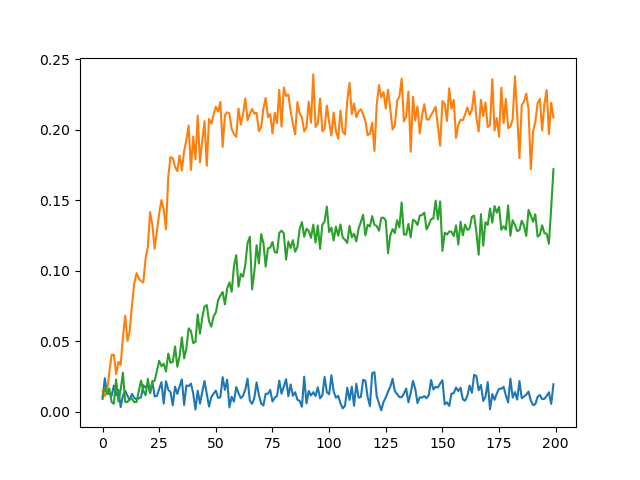
\includegraphics[scale=0.32]{../experiments/basic_demonstration/dependence_detection.png} }}%
	\qquad
	\subfloat{{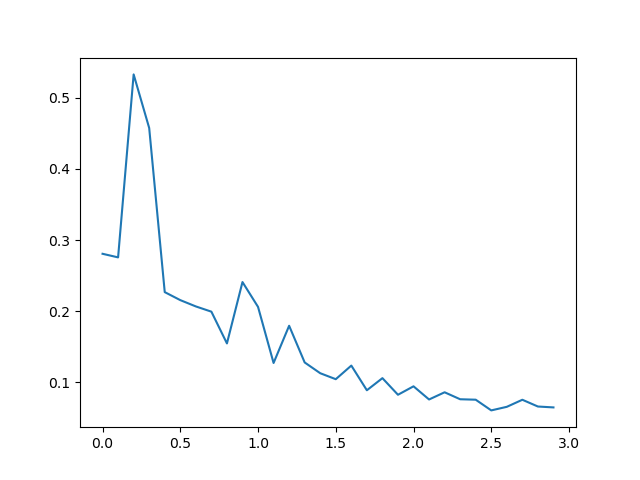
\includegraphics[scale=0.32]{../experiments/noise_effect/summary.png} }}%
	\caption{Left figure: KacIM evaluation for independent data (blue), additive (orange) and multiplicative (green) noise scenarios ($x$ axis - iteration, and $y$ - corresponding value of KacIM). Right figure: noise level ($x$ axis) vs final iteration KacIM value ($y$ axis). KacIM values for larger noise levels saturates as in tail of graph}
	\label{fig:experiments_simulation}
\end{figure}

Figure~\ref{fig:experiments_simulation} reflects KacIM values during iterative adaptation ($200$ iterations). In the case of independent data, both $x_{i}$ and $y_{i}$ ($d_{x} = 512$, $d_{y} = 4$) are sampled from gaussian distribution, independently. In the case of dependent data, an additive noise and multiplicative noise, the dependent variable is generated according to $y_{i} = sin(P x_{i}) + cos(P x_{i}) + \lambda \epsilon_{i}$ ($\lambda = 1.00$) and $y_{i} = (sin(P x_{i}) + cos(P x_{i})) \epsilon_{i}$, respectively, where $P$ is $d_{x} \times d_{y}$ random projection matrix, $\epsilon_{i} \sim N(0,1)$ and $\epsilon_{i} \perp x_{i}$.

When data is independent, both in additive and multiplicative cases, due to independence, estimator~\eqref{eq:estimator} is resistant to maximisation, and oscillates near zero. On the other hand, when the data is not independent, the condition~\eqref{eq:kac_theorem} is violated and maximization of estimator~\eqref{eq:estimator} is possible.
\paragraph{Noise variance effect} In this simulation we use the same additive noise setting as in previous paragraph, but evaluate all noise levels $\lambda \in [0.1, 3.0]$, with step $0.1$.
Figure~\ref{fig:experiments_simulation} empirically shows that value of KacIM  negatively correlates with noise level, and therefore the proposed measure is able not only to detect whether independence is present, but also to quantitatively evaluate it.

%Since in~\ref{alg:estimator_computation} we standartize data, KacIM is also scale-invariant (i.e. $\kappa(rx, ry) = \kappa(x,y)$), where $r>0$ is scale parameter.

\paragraph{Comparison with distance correlation} We also evaluated distance correlation~\cite{Szekely} on the same generated samples of data, comparing it with KacIM. From Figure.~\ref{fig:experiments_simulation_dcor} we see that as data dimensionality grows, for independent data, the values of measure not only is significantly larger than zero, but it also grows like values of measure of dependent data. This empirically demonstrates that distance correlation is affected by the curse of dimensionality. On the other side, KacIM even for larger dimensions oscilates near zero for independent data, and significantly deviates from zero for dependent data case, as indicated in right component of Figure.~\ref{fig:experiments_simulation_dcor}.



\begin{figure}%
	\centering
	\subfloat{{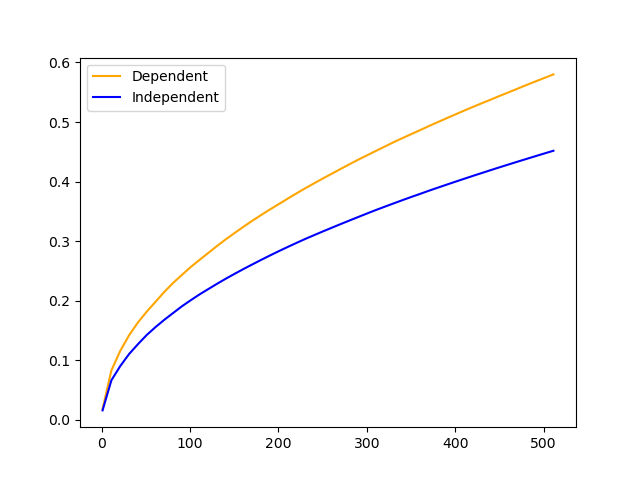
\includegraphics[scale=0.32]{../experiments/basic_demonstration/dependence_detection_dcor_dim.png} }}%
	\qquad
	\subfloat{{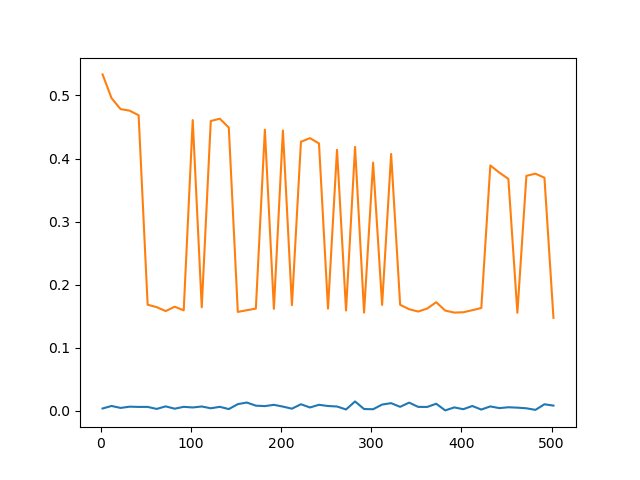
\includegraphics[scale=0.32]{../experiments/basic_demonstration/aaa_dependence_detection_kacim_by_dim_502.png} }}%

	\caption{The dimension of data is on the $x$ axis, and on $y$ axis is evaluation of distance correlation (left) and KacIM (right). Blue graph corresponds of independent data of dimension, indicated by $x$ axis, and orange one corresponds to dependent data.}
\label{fig:experiments_simulation_dcor}
\end{figure}

%\subsection{Feature selection}
%Shubham


\subsection{Feature extraction}

Previous work in the field of supervised feature extraction (also parralel field termed dimensionality reduction), which rely on dependency-based cost functions, include [?,?,?]. 

%Further we will extend [?,?] algorithms in the dimension of the dependence measure, as the parameter. In our reasoining, and formulations we will adopt Bayesian framework, embodied in this probability factorisation:
%P(S|A,S') = F()/



Let use denote by $T := (x_{i},y_{i})_{i=1}^{N}$ a supervised-learning dataset of $N$ pairs of $d_{x}$-dimensional inputs $x_{i}$, and $d_{y}$-dimensional one-hot-encoded outputs $y_{i}$.

In feature extraction experiments we will use a set of classification data sets from OpenML~\cite{OpenML2013}, which cover different domains.  We use $KacIM$ in order to conduct supervised linear feature extraction by seeking 

\begin{equation}
\label{eq:kim_feature_extraction}    
W^{*} = arg \max_{W} \kappa(Wx, y) - \alpha Tr\{(W^{T}W-I)^{T}(W^{T}W-I) \},
\end{equation}
where the regularisation term, controlled by multiplier $\alpha \geq 0$, enforces orthogonality of projection matrix $W^{*}$, and $Tr\{.\}$ denotes matrix trace operator.


In all the experiments~\eqref{eq:kim_feature_extraction} the cost function is optimised iteratively ($250$ iterations), simultaneously optimising parameters of KacIM ($\alpha$ and $\beta$) and projection matrix $W$.
After the optimisation, the feature extraction is conducted by $f(x) = W^{*}x$, where $x$ is original input vector, and $f$ are corresponding feature vector. 



We randomly split all the datasets in training and testing sets of equal size. % comparing unmodified inputs $x$, and features % of all possible dimensions up to $d_{x}$ with $10\%$ step.  
In our experiments we set $\alpha$ to $1.0$ to quickly ensure orthogonal projection matrices, and further proceed to dependence maximization stage. In order to quantitatively evaluate features, we use logistic regression-based classification accuracy, measured on the testing set.


We use two baselines: raw features (RAW column in Table~\ref{table:classification_accuracies}) and neighborhood component analysis~\cite{NIPS2004_42fe8808} (NCA column in Table~\ref{table:classification_accuracies}).  The purpose of these experiments is to provide the preliminary evaluation of the applicability of KacIM for feature extraction, hence we use rather basic cost function and comparative baselines.




The classification accuracies, reported in Table~\ref{table:classification_accuracies} demonstrate that KacIM-based feature extraction procedure (KacIMFE column) indeed allows to increase classification accuracy when applied to real data sets from different domains. In contrast to our feature extraction approach, NCA explicitly optimises for classification accuracy, rather than more abstract dependency of features $f(x)$ with dependent variable $y$.



\begin{table}	
	\centering
	\begin{tabular}{ |p{3cm}|p{2.0cm}|p{1.2cm}|p{1.7cm}|p{1.2cm}|  }
		%\hline
		%\multicolumn{5}{|c|}{Classification accuracies} \\
		\hline
		Dataset & $N$/$d_{x}$/$n_{c}$. & Raw & KacIMFE & NCA  \\
		\hline
isolet & (7797,617,26)   &  0.9261  &  0.9437  &  \textbf{0.9477} \\
madelon & (2600,500,2)   &  \textbf{0.6015}  &  0.5484  &  0.5685 \\
prnn-viruses & (61,18,4)   &  0.6452  &  0.9265  &  0.9355 \\
ionosphere & (351,34,2)   &  0.8807  &  0.9278  &  \textbf{0.9375} \\
micro-mass & (360,1300,10)   &  0.8778  &  \textbf{0.9282}  &  0.8944 \\
%CostaMadre1 & (296,37,2)   &  \textbf{0.8716}  &  0.8549  &  0.8378 \\
clean1 & (476,168,2)   &  0.7689  &  \textbf{0.9888}  &  0.9790 \\
%pc4 & (1458,37,2)   &  \textbf{0.8779}  &  0.8707  &  0.8683 \\
robot-failures-lp2 & (47,90,5)   &  0.4583  &  0.6067  &  0.5833 \\
waveform-5000 & (5000,40,3)   &  \textbf{0.8692}  &  0.8017  &  0.8516 \\
spambase & (4601,57,2)   &  0.6906  &  0.8285  &  \textbf{0.8705} \\
gina-agnostic & (3468,970,2)   &  \textbf{0.8512}  &  0.7894  &  0.8080 \\
scene & (2407,299,2)   &  0.8895  &  \textbf{0.9707}  &  0.9336 \\
tokyo1 & (959,44,2)   &  0.7250  &  0.8995  &  \textbf{0.9062} \\
one-hundred-plants-shape & (1600,64,100)   &  0.1013  &  \textbf{0.4913}  &  0.4688 \\		
		
		\hline
	\end{tabular}
	\caption{Classification accuracies. $N$ denotes full data set size, $d_{x}$ - input dimensionality, and $n_{c}$ - number of classes. In this table feature dimension is equal to a half of original input dimension. Best accuracies that are also statistically significant (Wilcoxon's signed rank test~\cite{Wilcoxon1992}, 25 runs, $p$-value threshold $0.01$) are indicated in bold text.}
	\label{table:classification_accuracies}	
\end{table}

\begin{comment}
\begin{table}	
	\centering
	\begin{tabular}{ |p{3cm}|p{2.0cm}|p{1.2cm}|p{1.7cm}|p{1.2cm}|  }
		%\hline
		%\multicolumn{5}{|c|}{Classification accuracies} \\
		\hline
		Dataset & $N$/$d_{x}$/$n_{c}$. & Raw & KacIMFE & NCA  \\
		\hline
		micro-mass  &  (360,1300,10)  &   0.88  &   0.93  &   0.89 \\
		ionosphere  &  (351,34,2)  &   0.88  &   0.92  &   0.94 \\
		spambase  &  (4601,57,2)  &   0.69  &   0.83  &   0.87 \\
		lsvt  &  (126,310,2)  &   0.67  &   0.68  &   0.78 \\		
		one-hundred-plants-texture  &  (1599,64,100)  &   0.62  &   0.77  &   0.80 \\
		tokyo1  &  (959,44,2)  &   0.72  &   0.89  &   0.91 \\				
		clean1  &  (476,168,2)  &   0.77  &   0.99  &   0.98 \\
		one-hundred-plants-shape  &  (1600,64,100)  &   0.10  &   0.48  &   0.47 \\	
		pc4  &  (1458,37,2)  &   0.88  &   0.87  &   0.87 \\
		madelon  &  (2600,500,2)  &   0.60  &   0.55  &   0.57 \\
		scene  &  (2407,299,2)  &   0.89  &   0.98  &   0.93 \\
		%gina\_agnostic  &  (3468,970,2)  &   0.85  &   0.80  &   0.81 \\
		isolet  &  (7797,617,26)  &   0.93  &   0.95  &   0.95 \\			
								
		\hline
	\end{tabular}
	\caption{Classification accuracies. $N$ denotes full data set size, $d_{x}$ - input dimensionality, and $n_{c}$ - number of classes. In this table feature dimension is equal to a half of original input dimension. }
	\label{table:classification_accuracies}	
\end{table}
\end{comment}


\subsection{Regularisation}
In regularisation experiments we investigate chest x-ray classification task. It is represented as binary classification data set, consisting of x-ray scans ($5216$ for training, and $642$ for testing), which should be classified as pneumonia or normal (e.g. Figure~\ref{fig:Pneumonia_dataset_examples}). As classifier we use \emph{ResNet18}, trained with batches of $128$ elements.
We denote classifier as $f(\phi(x|\theta_{0})|\theta_{1})$, where $\theta_{0}$ are bottleneck parameters, $\theta_{1}$ final (linear) layer parameters, and $x$ is $224\times 224$ input image.
For optimisation we use decoupled weight decay regularization optimizer~\cite{Loshchilov2019DecoupledWD} with learning rate set to $0.0002$, and weight decay parameter set to $0.00001$ ($7$ epochs).
We used the following data augmentations: random horizontal flip, random rotation (up to 10 degrees), color jitter.
 
\begin{figure}%
	\centering
	\subfloat{{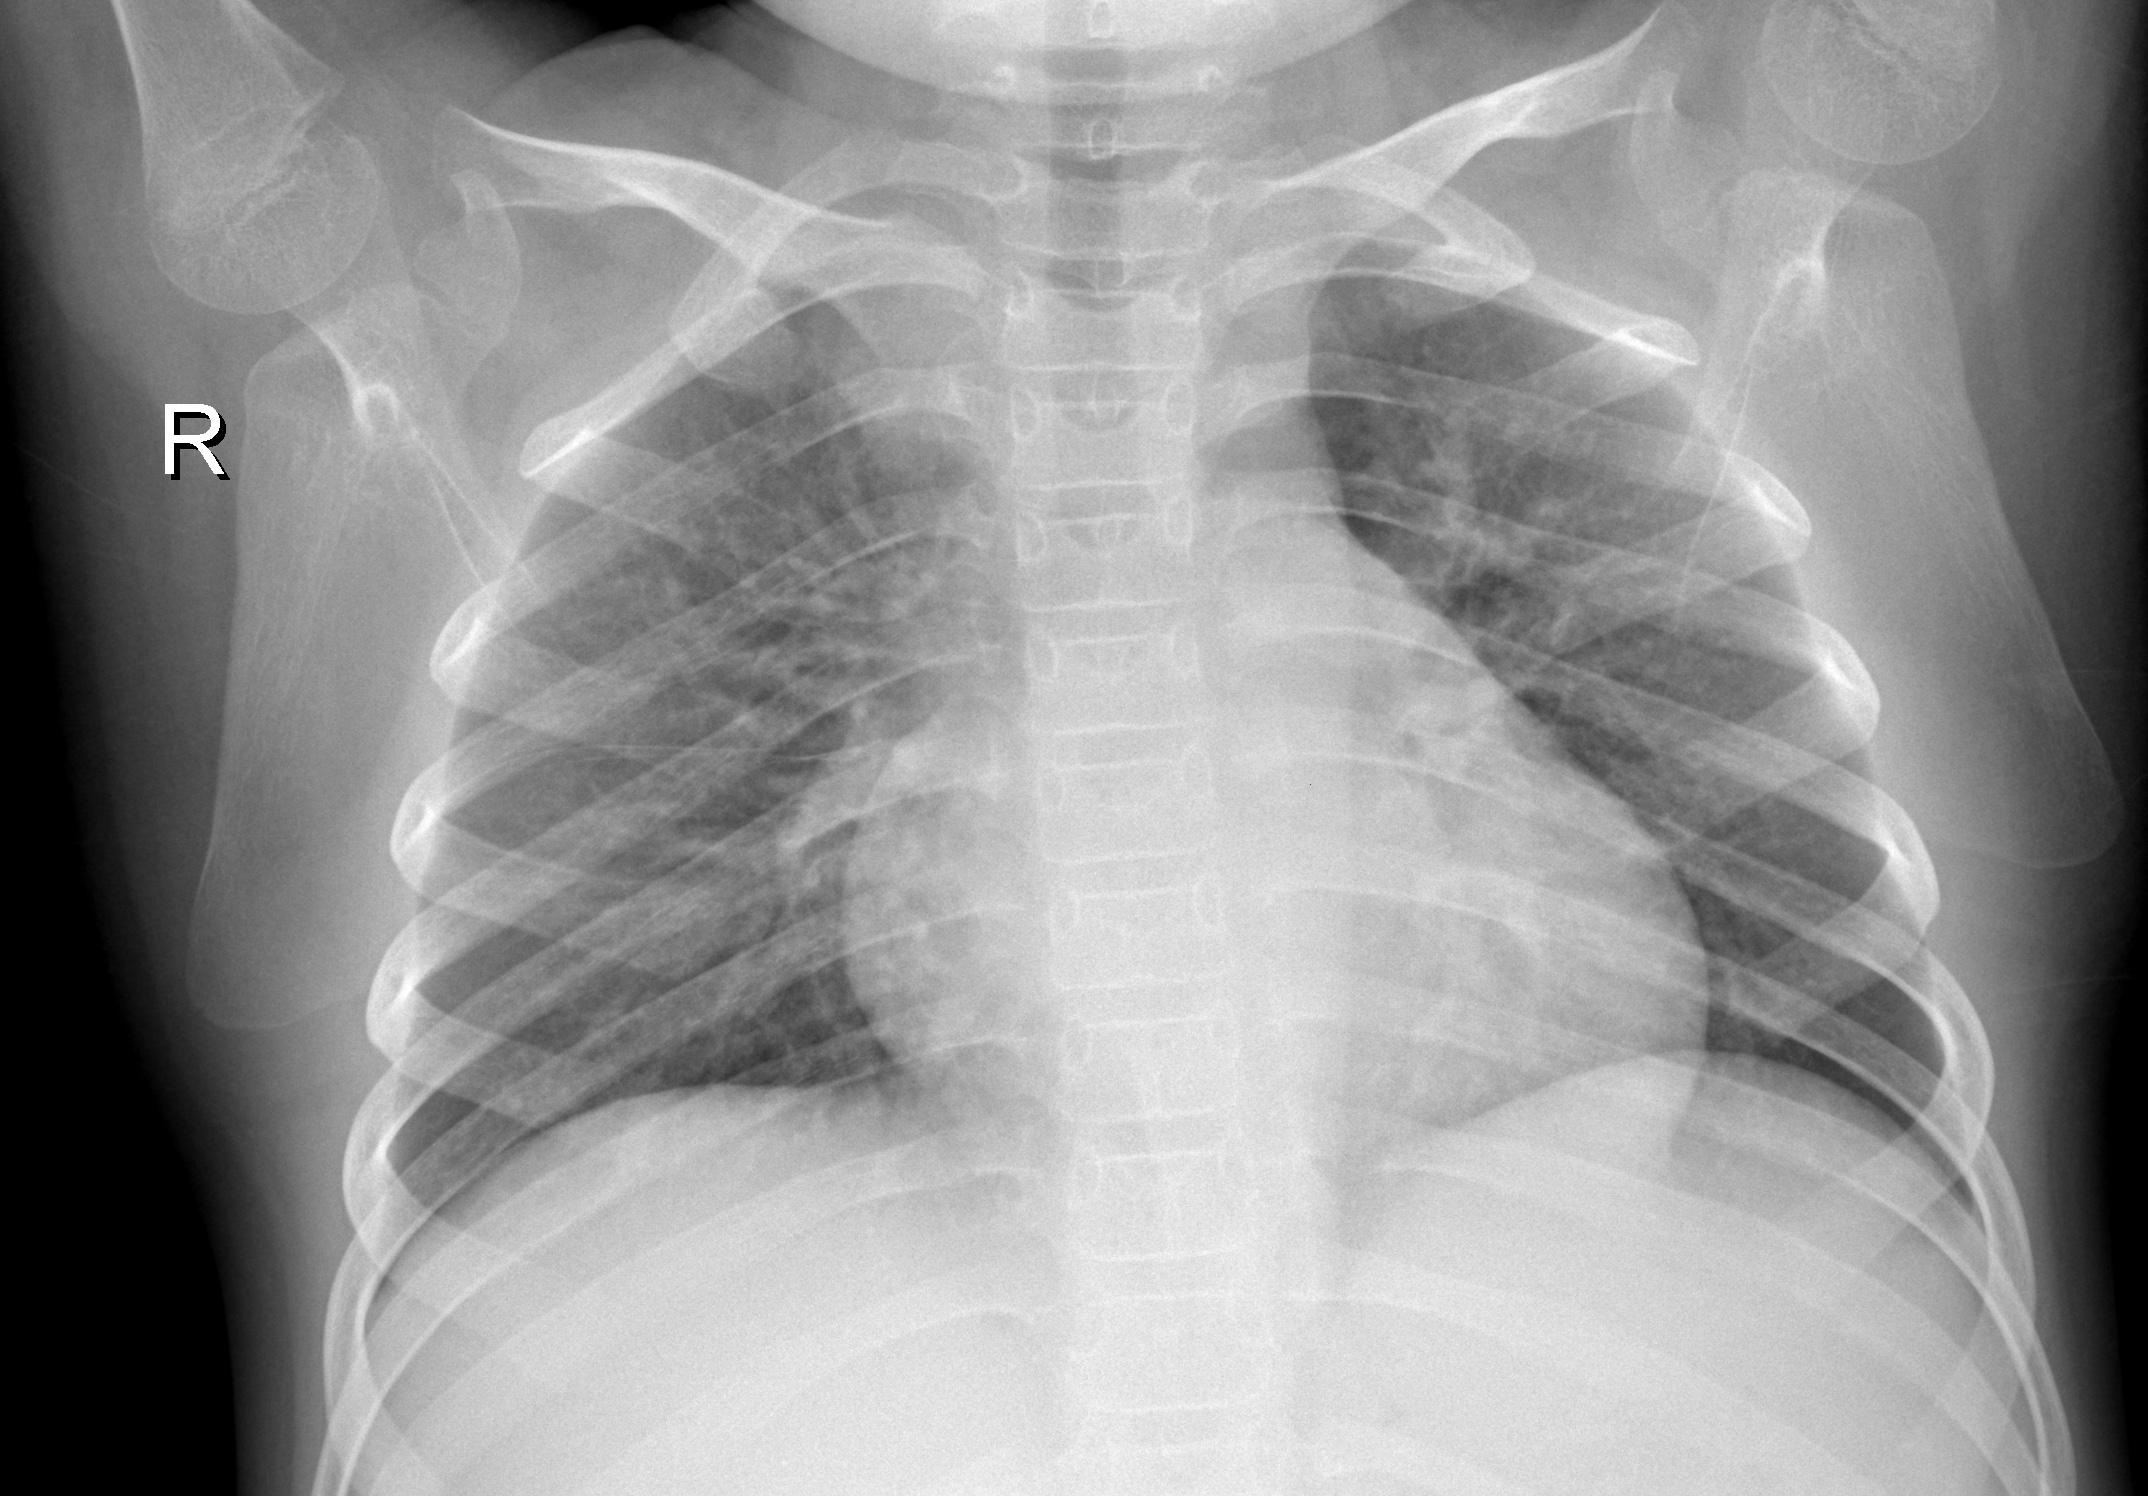
\includegraphics[scale=0.07]{./img/IM-0170-0001.jpeg} }}%
	\qquad
	\subfloat{{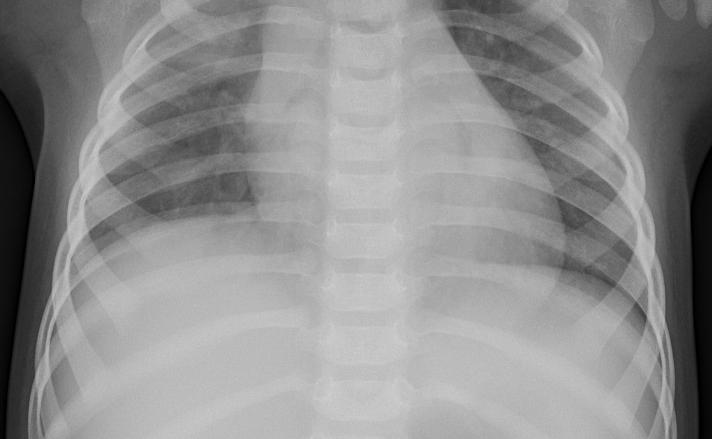
\includegraphics[scale=0.20]{./img/person1_bacteria_1.jpeg} }}%
	\caption{Left figure: example of healthy lung x-ray. Right: pneumonia.}
	\label{fig:Pneumonia_dataset_examples}
\end{figure}


We will investigate additive regularizer, which maximises depency of bottleneck the feature $\phi(x)$ and target variable $y$ (one-hot encoding): 


\begin{equation}
Cost(\theta_{0},\theta_{1}, W) := CE(f(\phi(x|\theta_{0})|\theta_{1}),y) - \beta \kappa(W\phi(x|\theta_{0}),y),
\end{equation}

\noindent where $CE(.,.)$ is cross-entropy loss, $W$ is $32\times 512$ projection matrix, and $\beta \geq 0$ is regularisation parameter (in our experiments $\beta = 0.1$).

\begin{table}	
	\centering
	\begin{tabular}{ |p{4cm}|p{2cm}|}
		%\hline
		%\multicolumn{5}{|c|}{Classification accuracies} \\
		\hline
		Mode & esting  \\
		\hline
		Without regularisation   &    0.8338 \\		
		\hline
		With regularisation  &   0.8427 \\		
		\hline
	\end{tabular}
	\caption{Classification accuracy comparison of regularised and not regularised model (pneumonia dataset).  }
	\label{table:regularisation_classification_accuracies}	
\end{table}

The results of classification accuracy without and with aforementioned regularisation is reported in Table~\ref{table:regularisation_classification_accuracies}.


\section{Conclusion} 

\label{section:conclusion}
In this article we propose statistical dependence measure, KacIM, which corresponds to the $L^{\infty}$ norm of the absolute value of difference between joint characteristic function and the product of marginal ones. The proposed measure, in theory can detect both linear and non-linear statistical depdendence between a pairs of random variables of possibly different dimension, extended to various known statistical generalisations (e.g. reproducing kernel Hilbert spaces, multivariablity), machine learning scenarios (e.g. feature extraction, regularisation, among others), and is empirically tractable on these problems. On the other side, it raises a corresponding set of unanswered questions, both theoretical and empirical. For example, the interpretability when it approaches its maximal value remains insufficiently clear, however empirical experiments with simulated data reveals, that increasing independence between two random variables is reflected in a decreasing trend on the estimated values of the proposed dependence measure. In contrary to e.g. HSIC or distance correlation, the estimation of the porposed measure is iterative optimisation process. Therefore, parameter initialization, meta-parameter (e.g. stopping criteria, batch size) selection are needed in order to evaluate it efficiently.

Beside demonstrated applications in Section~\ref{section:experiments}, the proposed measure is differentiable and thereby can be integrated with various modern deep-learning methods, applied to high-dimensional and structured data. From empirical point of view, we see exploration of KacIM in causality, information bottleneck theory, self-supervised learning, and other modern problems, where dependence measures define a criterion of optimisation, as important future work. %We also would like to note, that exhaustive survey of measures of statistical dependence, accompanied with open-source code repository, would be helpful both for the theorists and for practicioneers.

\begin{comment}
....

Although we formulated and analysed KacIM for bivariate vectorial case, similarly it can be generalised for multivariate case. In addition, since characteristic functions are defined for matrices, graphs, and other objects \cite{?}, the proposed dependence measure can be extended to those objects as well, which is potential direction of future research of KacIM.



Conducted empirical analysis show, that KacIM can detect and measure statistical independence for non-linearly related, high-dimensional data, and that it can be applied for feature extraction and DNN regularisation and improve model's performance on real data sets. On the other side, direct applications of the proposed statistical dependence measure in the areas of causality, information bottleneck, and other domains where not explored in this study, and left for the future work, as well as its  important properties (e.g. interpretability, limit distribution).
\end{comment}

\section{Acknowledgements}

We sincerely thank Dr. Pranas Vaitkus, Dr. Linas Petkevi\v{c}ius, and colleagues from Neurotechnology for discussions. We also thank Neurotechnology for supporting this research.

%\subsection{KacIM for information bottleneck}
%\subsection{Canonical component analysis, independent component analysis}
%\subsection{Causal inference}
%\subsection{Electroencephalography (?)}
%\section{Notes}
%Compare with  mutual information.


%\bibliographystyle{apalike}
\bibliographystyle{unsrt}

{\footnotesize
\bibliography{bibliography}}

% https://arxiv.org/pdf/2104.06612.pdf

%\begin{thebibliography}{}
%\bibitem{KacTheorem} David Applebaum, B.V. Rajarama Bhat, Johan Kustermans, J. Martin Lindsay, Michael Schuermann, Uwe Franz: Quantum Independent Increment Processes I: From Classical Probability to Quantum Stochastic Calculus
%\end{thebibliography}

\end{document}
